\documentclass[11pt,letterpaper]{article}
\usepackage[margin=0.75in]{geometry}
\usepackage[T1]{fontenc}
\usepackage{lmodern,microtype,amsmath,amssymb,booktabs,array,float,graphicx,hyperref}
\hypersetup{hidelinks}
\setlength{\parindent}{0pt}
\setlength{\parskip}{0.4em}
\title{\textbf{Learning to Allocate Risk in Options Markets}\\[0.4em]\large Contextual Bandits for Trade Sizing and Q-Learning for Capital Allocation}
\author{Adam Kreitzman and Soo Xin Yang\\MFE 230Z: Deep Learning in Finance}
\date{20 October 2026}
\begin{document}
\maketitle
\begin{abstract}
We study reinforcement learning for two exposure decisions in equity options: sizing individual trades with contextual bandits and allocating capital between strategies with fitted Q-learning. Actual-contract simulations combine approximately 30-day, 25-delta put pairs with short ATM straddles selected by persistent realized-minus-implied volatility. During January 2022--August 2025, learned entry sizing raises annualized excess Sharpe from 1.055 to 1.263 for put pairs and from 0.990 to 1.041 for straddles, relative to full sizing. Combining both learners raises Sharpe from 1.088 to 1.726 in a four-way comparison. With bandit entries, Q also exceeds rolling mean--variance allocation: 1.726 versus 1.519. Interpretation connects entry decisions to completed profitability and volatility, and strategy allocation to the changing reward for straddle risk. Statistical uncertainty and assumed execution quality qualify these historical results.

\end{abstract}
\subsection*{1. From a useful signal to an exposure decision}
Suppose AMD and NVDA face similar news, but AMD options become unusually expensive relative to NVDA options. Selling the richer options and buying the cheaper ones expresses a view about the relative price of volatility. Daily stock hedges reduce immediate directional exposure, and initial vega matching reduces sensitivity to a common small change in implied volatility. The trade still carries risk: related stocks can experience different events, and option premiums may correctly reflect those differences.

Our starting point is Ning and Lee's equity-pairs framework [1], which separates constructing a spread from learning how to trade it. We carry that distinction into options. First, we ask whether an economic rule produces useful historical trades under explicit contract and funding assumptions. We then ask whether learning improves the amount of capital assigned to those opportunities. A profitable signal and a useful allocation policy are separate findings.

\begin{figure}[H]\centering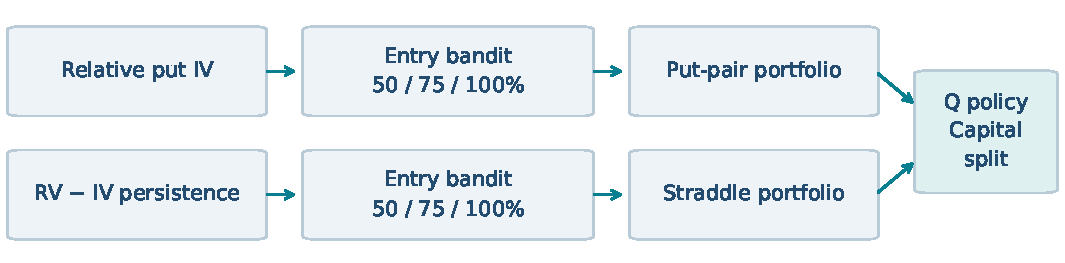
\includegraphics[width=\textwidth,height=127pt,keepaspectratio]{paper/unified_learning_2026_10_16/figures/learning_pipeline.pdf}\caption{Two exposure decisions. Entry policies size proposals within each signal; a separately fitted Q policy chooses the capital split between funded strategy indices.}\end{figure}
The original relative-volatility strategy remains the foundation of this paper. We add a second signal---persistent realized-minus-implied volatility---and a second learning decision: allocating capital between the resulting strategies. Entry bandits choose individual trade sizes; fitted Q-learning chooses the strategy mix. Both reporting periods, 2018--2021 validation and January 2022--August 2025 evaluation, remain visible throughout.

\clearpage
\section*{2. What we take from the motivating paper}
\subsection*{Construct the opportunity, then learn how to trade it}
Ning and Lee [1] study how to construct and trade mean-reverting equity spreads. If the two stock prices are S₁ and S₂, they form X = S₁ - B S₂. They choose the hedge coefficient B by grid search to minimize empirical mean-reversion time: the average duration from a significant local extreme to the next mean crossing. Spread formation is empirical; it does not first impose an Ornstein--Uhlenbeck (OU) model.

For trading, they use tabular Q-learning. The state records recent spread moves by direction and magnitude. Actions buy, hold or sell a unit, subject to current inventory; the agent enters a long spread and later closes it. Its reward favors buying below and selling above an equilibrium mean, with a transaction-cost term. Q-values combine immediate reward with the estimated value of later decisions.

The agent trains on 10,000 simulated one-year OU paths because the reward requires a known equilibrium mean. The market study forms ten US pairs in 2022 and trades them in 2023. The combined method exceeds the Distance Method and OU benchmarks on their reported daily Sharpe measure. Those daily figures are not directly comparable with our annualized options ratios.

\subsection*{What the evidence establishes---and leaves open}
One trading year gives limited evidence across regimes. Formation and trading policy also change together, so their comparison does not isolate Q-learning's contribution. The simulated equilibrium is known; a real relationship's equilibrium can shift. Finally, a cost term in a reward does not by itself establish net execution quality or scalability. These issues motivate our use of actual contracts, explicit cash flows, several market years and controlled exposure comparisons.

\begin{center}\small\resizebox{\textwidth}{!}{\begin{tabular}{lll}\toprule
Design choice & Motivating study & Our extension\\\midrule
Economic object & Equity-price spread & Relative option IV; persistent RV - IV\\
Policy experience & Simulated mean reversion & Completed historical trade paths\\
Learned decision & Spread entry and exit & Entry size; then strategy allocation\\
Comparison & Different spread-trading methods & Shared proposals; separate learning layers\\
\bottomrule\end{tabular}}\end{center}
We retain the separation between finding a spread and learning how to trade it. We change the instrument, reward and decision problem. A successful sizing policy does not establish that the original paper's trading algorithm transfers unchanged to options. Our later Q experiment is closer to its sequential question: present allocations affect holdings, subsequent resizing costs and future choices.

The early ATM-volatility proxy results gave us reason to investigate further, but weakened when simulated with actual contracts. Strike-specific payoffs, daily hedge errors and costs were absent from the simple IV-versus-future-RV proxy. We investigated maturity, position on the option smile and additional predictors. Approximately 30-day, 25-delta puts became the retained relative-volatility configuration.

Bell et al. [6] develop AlphaGlass, which maps characteristics into additive signals with sparse interactions and optimizes portfolio objectives directly. Their interpretable characteristic-based portfolio choice connects to our Sharpe-based sizing and policy diagnostics. We study a different decision structure: sizing actual option trades and allocating between strategy books through fitted Q-learning.

\clearpage
\section*{3. What the option trade actually does}
A put gives its buyer the right to sell stock at a specified strike. Our retained pair strategy selects out-of-the-money puts near 25 delta and approximately 30 days to expiry. At delta -0.25, a small \$1 rise in the stock initially lowers the put's value by about \$0.25 per share. Delta measures price sensitivity; it is not an exact probability of exercise.

Implied volatility (IV) is the volatility input that makes an option-pricing model reproduce a quoted price. Higher IV generally means a more expensive option, holding other inputs fixed. Realized volatility (RV) describes how much the stock actually moves. Selling an option can be attractive when the premium compensates for those future movements; buying can be attractive in the opposite situation. Future RV is unknown at entry.

\subsection*{A worked example: matching vega and hedging delta}
Vega measures the change in option value when IV rises by one percentage point---for example, from 30\% to 31\%. The table reports total position vega; each option contract represents 100 shares. These are illustrative numbers, not an observed trade.

\begin{center}\small\resizebox{\textwidth}{!}{\begin{tabular}{llll}\toprule
Position & Contracts & Total vega per IV point & Initial stock hedge\\\midrule
Buy A puts & +100 & +\$450 & Buy 2,500 shares\\
Sell B puts & -150 & -\$450 & Short 3,750 shares\\
\bottomrule\end{tabular}}\end{center}
Each A contract has \$4.50 of vega and each B contract \$3.00. Buying 100 A contracts and selling 150 B contracts therefore balances +\$450 against -\$450. An equal one-point IV increase approximately cancels at entry. Both puts initially have delta -0.25 per share: the long puts require buying stock, while the short puts require selling it. Equal option counts would generally fail to balance vega.

If A's IV instead rises by two points while B's rises by one, the initial vega approximation gives a \$900 gain on A and a \$450 loss on B: a \$450 net gain before other effects. This is a local approximation to changes in option marks, not a formula for profit earned by holding to expiry. We match vega at entry and adjust stock delta hedges daily; we do not continuously restore vega neutrality.

\subsection*{What earns or loses money?}
After delta hedging, returns still depend on the stock's path. Gamma describes how delta changes as stock moves; theta describes time decay. A long put's movement gains must compensate for time decay and costs. A short option earns decay but loses from sufficiently large moves. The leading small-interval terms are

\[\Delta P_{\rm hedged}\approx\frac{1}{2}\Gamma(\Delta S)^2+\Theta\Delta t+V\Delta IV.\]
Our backtester records option marks, terminal payoffs and stock cash flows. It does not replace them with ``realized volatility minus implied volatility.'' Initial vega neutrality also leaves differences in gamma, jump exposure and responses to market stress. In the approximation, V and the IV change use the same volatility-point units.

\clearpage
\section*{4. Finding the relative-volatility signal}
\subsection*{Relative richness across related names}
For each pair, we compare the IV difference D = IV\_A - IV\_B with its latest 252 trading sessions, requiring 63 observations. At the upper quintile we sell A's relatively high-IV put and buy B's; at the lower quintile we reverse direction. Historical ranking matters: a ten-point gap means something different for a pair usually five points apart than for one usually fifteen points apart.

\begin{figure}[H]\centering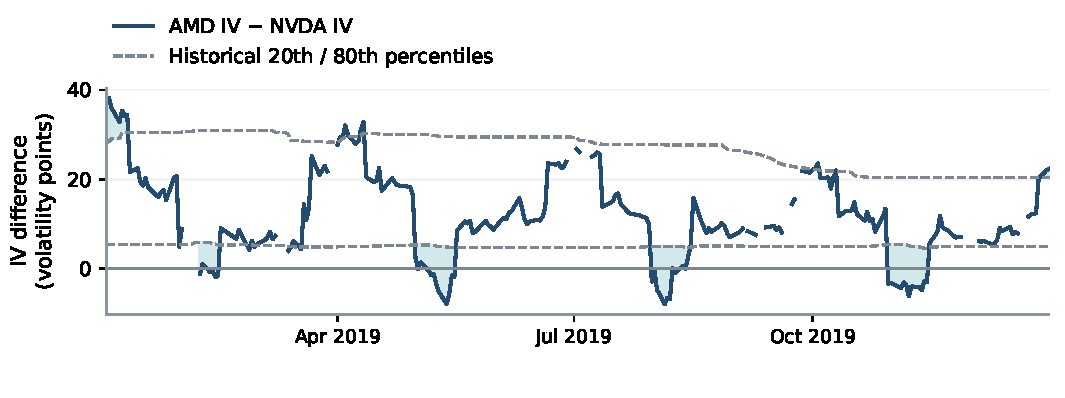
\includegraphics[width=\textwidth,height=191pt,keepaspectratio]{paper/unified_learning_2026_10_16/figures/signal_example.pdf}\caption{AMD minus NVDA selected-put IV in 2019. Shading marks excursions outside historical percentile boundaries, not executed trades. Gaps are unavailable quotes. Daily contract selection makes this a signal series, not the mark of one held contract.}\end{figure}
Monthly formation requires 126-session return beta between 0.85 and 1.15 and correlation of at least 0.5. The proposed direction must also show positive historical profit per initial vega over 91 and 365 calendar days, with 21 and 63 completed observations. These are simulated standalone candidates, not just funded fills. A trade entered yesterday with a month left cannot contribute its eventual profit today.

\subsection*{Why an extreme is not enough}
Beta measures the scale of one name's response to the other; correlation measures how consistently they move together. Neither guarantees that their option prices should behave alike. The relatedness screens keep the comparison among reasonably similar names without treating relatedness as the trading signal.

The profitability memory adds a different economic question: has this direction recently paid for the premium and hedging costs? We are looking for an unusually wide IV difference in a direction with evidence of structural relative richness, rather than assuming every large gap must revert. The memory and completed-count conditions are selected rules, shared across all put sizing controls.

The chart follows each day's selected contract. After entry, the simulator holds the purchased and sold contracts rather than replacing them when daily selection changes. Profit therefore depends on their realized option and hedge cash flows. A temporary narrowing of the displayed IV gap is neither required nor sufficient for a profitable expiry trade.

\clearpage
\section*{5. A second signal: persistent volatility richness}
\subsection*{Why sell the names where realized volatility keeps disappointing?}
Some names repeatedly realize less movement than their option premiums imply. The second signal uses that persistence within each name rather than requiring a second company with offsetting vega. It asks whether an observed premium has been sufficiently persistent to justify selling the next roughly 30-day volatility exposure. The economic idea is related to Goyal and Saretto [2]; the new question here is how to size and allocate around it.

For every historical candidate, subtract entry ATM-call IV from the annualized RV measured after the next-session entry close through that contract's expiry. Only after the outcome finishes can it join the signal history. Average those completed RV - IV observations over the preceding 365 calendar days, requiring 126. Rank eligible names each day and sell the bottom 10\%.

\[M_{i,t}=\operatorname{mean}_{u:\,t-365<T_u<t}\left(RV_{i,u\to T_u}-IV^{\rm ATM\ call}_{i,u}\right).\]
For illustration, a name whose completed outcomes average RV 26\% against entry IV 34\% has memory -8 volatility points. A name averaging -2 points ranks less rich under this rule, although neither figure guarantees a profitable new short. Ranking is cross-sectional: bottom decile means the lowest eligible memories, not a fixed requirement that the premium exceed eight points.

\subsection*{Why a straddle, and what risk does it sell?}
ATM means the strike is near the current stock price. We sell an ATM call and put with the same name, strike and expiry, then adjust the stock delta hedge daily. This collects premium against movement in either direction. At full size, \$450 is the combined call-and-put vega budget. The position is short gamma and vega: quiet realized paths can support carry, while jumps and changing uncertainty can generate large losses. It is not vega neutral.

\begin{center}\small\resizebox{\textwidth}{!}{\begin{tabular}{lll}\toprule
Economic distinction & Relative put pair & ATM straddle\\\midrule
Comparison & Current gap versus pair history & Completed RV - IV versus other names\\
Exposure & Buy one put; sell another & Sell call and put on one name\\
Initial vega & Approximately offset across names & Net short\\
Main challenge & Different realized paths and events & Premium income versus movement risk\\
\bottomrule\end{tabular}}\end{center}
The signal retains ATM-call IV even though execution uses a straddle. It ranks a difference in annualized volatility units, not squared variance and not an exact option-return forecast. The actual-contract ledger determines profitability after premiums, hedging, costs and financing. This distinction prevents the ranking target from being mistaken for simulated profit.

The two signals consequently offer different portfolios. The pair trade targets relative option richness with initial vega offset; the straddle accepts market-volatility exposure to collect a persistent premium. Their different dollar profits and risk make capital allocation a separate decision from either trade's entry size.

\clearpage
\section*{6. Explaining the straddle account's profits}
The straddle signal forecasts persistent volatility richness. Its economic interpretation should also agree with the profits recorded by the backtester. We examine 2,599 executed straddle cohorts from January 2018 through 29 August 2025, retaining the learned sizing policy. This full-history attribution explains the straddle sleeve; it is separate from the later-period comparisons of learning policies.

\begin{figure}[H]\centering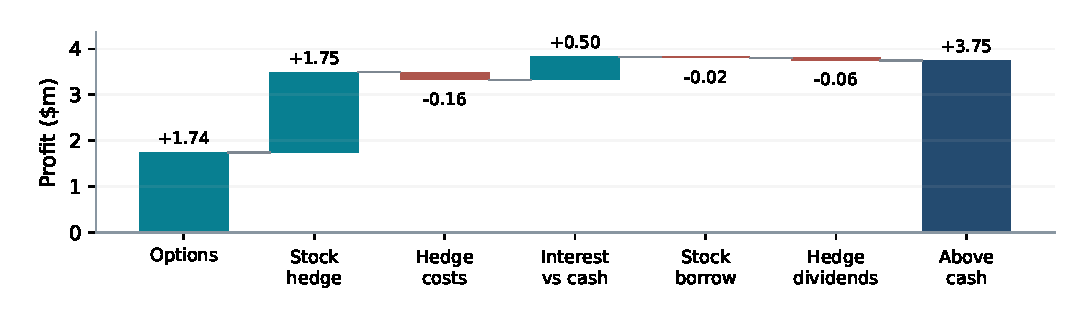
\includegraphics[width=\textwidth,height=200pt,keepaspectratio]{paper/unified_learning_2026_10_16/figures/straddle_bridge.pdf}\caption{Full-history straddle account, January 2018--August 2025. The option and stock components are read together; the remaining cash flows reconcile them to profit above cash.}\end{figure}
Options after option charges earned \$1.74 million; stock hedges before hedge costs earned \$1.75 million. Together they earned \$3.49 million, reconciled to \$3.75 million above cash after the remaining costs, dividends and financing. Positive profits in both components do not establish two independent sources of alpha. Option marks contain time decay, price moves and volatility revaluation; the stock hedge is held to offset option delta.

\begin{figure}[H]\centering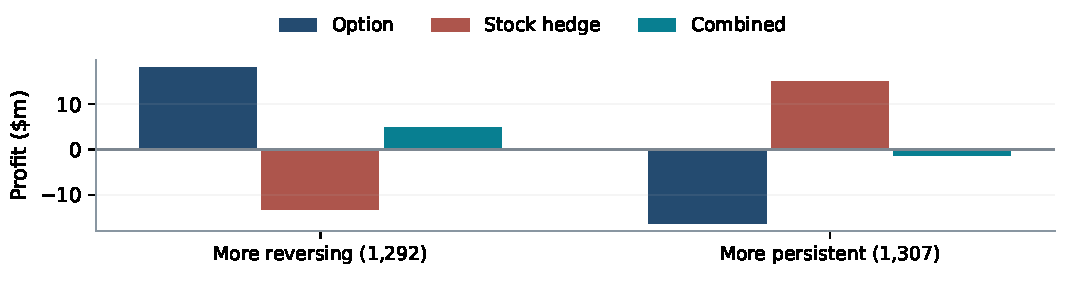
\includegraphics[width=\textwidth,height=200pt,keepaspectratio]{paper/unified_learning_2026_10_16/figures/straddle_paths.pdf}\caption{The same 2,599 cohorts grouped by their completed price paths. Combined profit includes option charges but precedes stock-hedge charges, dividends and financing. The grouping is descriptive.}\end{figure}
A short straddle has negative gamma. After a rising stock price, the delta hedge generally buys shares; after a fall, it sells. Continuing moves can reward the stock position while creating a larger option loss. Reversals can hurt the hedge while the option retains premium. In these cohorts, more reversing paths earn \$4.78 million together; more persistent paths lose \$1.29 million. The combined result is the relevant economic object.

Path persistence is the absolute entry-to-exit log return divided by the sum of absolute daily log returns. Values at or below 0.20 define the more reversing group. This grouping uses the completed path to explain results; it is not an available entry feature or a new trading rule.

\clearpage
\section*{7. Relating implied volatility to realized outcomes}
If the strategy earns a premium for selling movement risk, entry IV versus subsequent RV should help organize its outcomes. The diagnostic separates the same 2,599 cohorts by realized path and whether entry straddle IV exceeds the volatility subsequently realized. Both path groups have positive aggregate combined profit when IV exceeds RV and negative profit when it does not.

\begin{figure}[H]\centering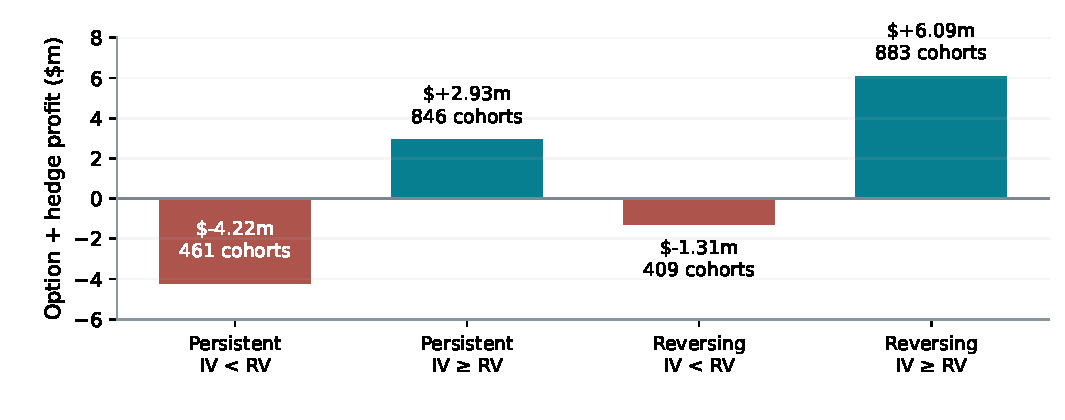
\includegraphics[width=\textwidth,height=200pt,keepaspectratio]{paper/unified_learning_2026_10_16/figures/straddle_ivrv.pdf}\caption{Combined option and hedge profit by completed price path and entry IV versus subsequent RV. These are realized-outcome groups, not new entry screens; totals depend on counts and sizes.}\end{figure}
\begin{center}\small\resizebox{\textwidth}{!}{\begin{tabular}{lllll}\toprule
Price path & IV vs RV & Trades & Profit (\$m) & Mean profit / premium\\\midrule
More persistent & IV < RV & 461 & -4.22 & -36.9\%\\
More persistent & IV ≥ RV & 846 & +2.93 & +13.0\%\\
More reversing & IV < RV & 409 & -1.31 & -15.3\%\\
More reversing & IV ≥ RV & 883 & +6.09 & +25.4\%\\
\bottomrule\end{tabular}}\end{center}
Entry IV here is the common annualized European, dividend-escrow volatility that reprices the combined call-and-put entry midpoint premium. Subsequent RV is the square root of 252 times mean squared daily log returns, from entry close to actual exit close, without subtracting the sample mean. The signal itself continues to use ATM-call IV; the common straddle IV is only an attribution measure.

The relation is not an exact profit identity. There are 220 losing cohorts even with entry IV above subsequent RV. Discrete delta hedging, jumps, changing gamma and execution charges matter. Calendar-time annualization changes 69 IV--RV classifications, and a dividend adjustment changes six; three cohorts exited early. The normalized profit column also does not match risk exposure across trades.

These are explanations using realized outcomes, not forecasts. They support the economic motivation for a completed-outcome RV - IV memory without showing that today's IV--RV gap is known in advance. They also clarify why a positive historical straddle return alone does not establish alpha after compensation for volatility risk.

\clearpage
\section*{8. Reading actual option and hedge paths}
Two contrasting historical cohorts make the accounting concrete. The left column was selected for a large stock-hedge gain; the right for a large hedge loss. Each panel uses the stock position already carried into that session, followed by the hedge adjustment at the close. These illustrations are deliberately selected examples, not representative performance estimates.

\begin{figure}[H]\centering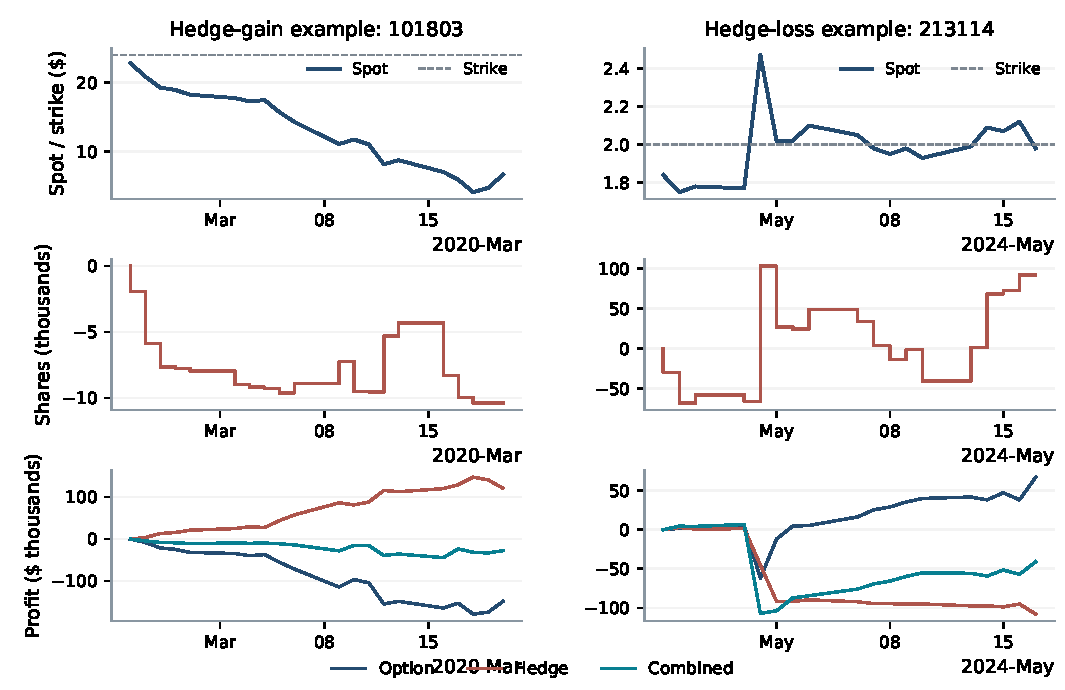
\includegraphics[width=\textwidth,height=200pt,keepaspectratio]{paper/unified_learning_2026_10_16/figures/straddle_examples.pdf}\caption{Two selected cohorts: a large hedge gain (left) and loss (right). Rows show spot versus strike, shares carried into each session, and cumulative option, stock and combined profit. Security IDs are stable identifiers.}\end{figure}
The stock hedge is not an independent trend strategy. A session's stock profit is shares carried into the session multiplied by the price change; the next close's shares control subsequent exposure. The lower panels therefore show the option and stock profits together. Their offset explains why neither the sign of hedge profit nor option premium retained can establish the profitability of a delta-hedged short.

The attribution also puts a limit on the gamma-versus-theta shorthand. We record actual option marks, stock hedge cash flows and costs rather than infer profit from one constant gamma or an unweighted RV - IV difference. A Greek expansion is useful intuition, but the ledger is the profit measure. Appendix F describes the recovered-quote reconciliation and the scope of reproduction.

\clearpage
\section*{9. Building the actual-contract backtester}
Historical option quotes, stock prices, rates and dividends come through WRDS. Each source strategy starts with \$10 million. Signal-date contracts trade in the following session if quotes and account checks permit. At full size, put pairs target \$450 vega per IV point on each leg; straddles target \$450 across call and put together. Whole contracts are rounded; put pairs allow an initial vega mismatch of no more than 10\%.

\subsection*{Daily marks, hedges and cash flows}
Options normally remain until expiry. At each close, we mark the existing option and stock positions, record cash flows and then rebalance stock delta. The next day's hedge profit uses the stock held after that rebalance. Final option payoffs and hedge unwinds complete the trade. Trading the same name on later dates is possible subject to existing inventory and risk checks.

Buying hedge stock debits cash; selling it credits cash. The cash balance earns the prior available benchmark rate, with negative cash paying that rate plus one percentage point annually. Short-stock borrow adds 0.30\% annually on short notional. Stock dividends are separate signed cash flows: a long holder receives the dividend and a short holder owes it. The ex-dividend stock-price drop does not replace that cash payment.

Option fills use midpoint plus an adverse charge of 0.10 IV point times traded vega and \$0.03 per contract; stock turnover costs one basis point. Expiry settlement has no option fill charge. Inventory, reserve, stress and quote checks determine admission. A request for less size can pass a pair limit and leave capacity for a later proposal. Appendix A defines the checks; they are research assumptions rather than broker margin.

\subsection*{What stays fixed, and what updates?}
\begin{figure}[H]\centering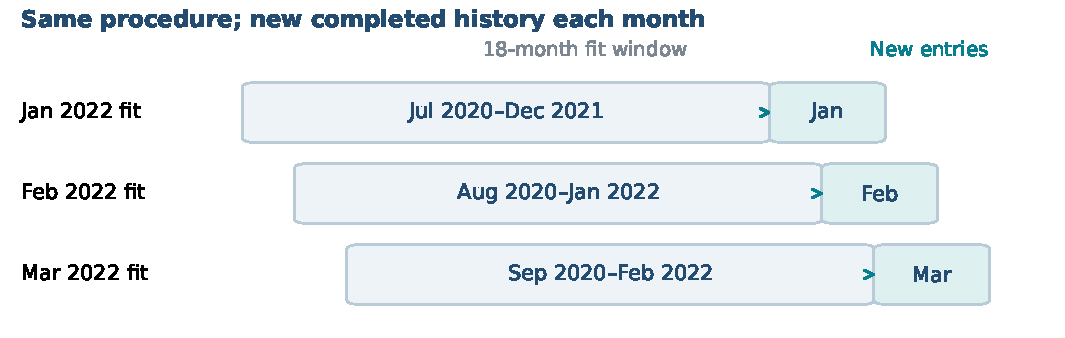
\includegraphics[width=\textwidth,height=162pt,keepaspectratio]{paper/unified_learning_2026_10_16/figures/refit_timeline.pdf}\caption{Monthly put-policy refitting. Only completed outcomes whose signal dates fall in the displayed 18-month window enter each fit. The selected model settings remain fixed; the tree and size assignments update.}\end{figure}
The put inputs, 18-month fitting window, tree settings and 50/75/100\% action menu remain fixed while the tree and size map refit monthly. Only outcomes completed before a fit enter training. A finished March trade can inform an April fit; an unfinished outcome cannot. Straddle and Q fits follow the same timing principle with their own windows. Accounts continue across the 2022 reporting boundary with accumulated cash and positions.

All Sharpe ratios annualize daily returns above cash. Dollar profit subtracts the increase in the continuing cash benchmark; Appendix E defines the metrics precisely.

\clearpage
\section*{10. Selecting information and training history}
The put learner's baseline 27 inputs describe spread rank, IV and trailing RV, beta and correlation, expiry, the CBOE Volatility Index (VIX), costs and completed profitability. Availability flags identify missing fields. Future trade profits are training outcomes, never current inputs.

\subsection*{A candidate measure of relative richness}
One additional block compares squared IV with forecast annualized variance. Its forecast uses exponentially weighted squared daily returns, with a 20-session half-life and at least 63 observations. Multiplication by 252 annualizes the estimate. The block adds the spread, a historical z-score and forecast-to-implied variance ratio, with availability flags.

\[\text{Variance spread}=IV^2-\widehat{\sigma}_{\rm RV}^{\,2}.\]
IV of 40\% and forecast RV of 30\% give 0.40\ensuremath{^2} - 0.30\ensuremath{^2} = 0.07, a variance difference rather than seven volatility points. A downside put also reflects skew, so this feature is not a clean underlying variance-risk-premium estimate. The EWMA block is a tested addition; it is not part of the retained 27-input put baseline.

\begin{figure}[H]\centering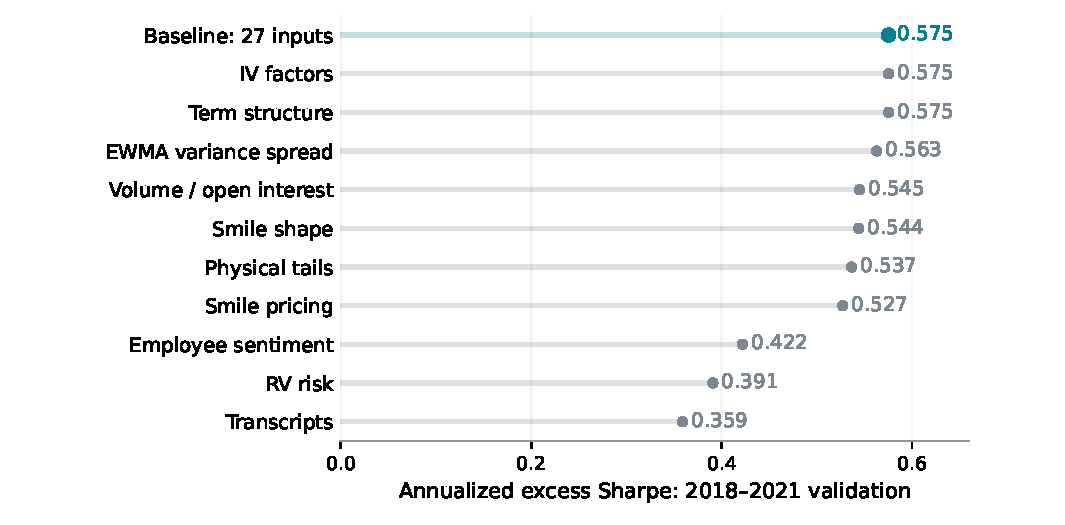
\includegraphics[width=\textwidth,height=253pt,keepaspectratio]{paper/unified_learning_2026_10_16/figures/feature_validation.pdf}\caption{Original feature exploration at the 18-month baseline. Scores use 2018--2021 validation and the archived \$345 million research account; funded policy comparisons use \$10 million. The three highest scores tie exactly.}\end{figure}
We rank 33 archived screened configurations by 2018--2021 validation excess Sharpe within the established 30-day, 25-delta design. Feature, window and action-menu experiments form this grid. Baseline, IV-factor and term-structure scores tie exactly at 0.575; alphabetical configuration ordering retains the baseline. The selected specification has 27 inputs, an 18-month window and 50/75/100\% sizes.

Archived selection scores use a \$345 million research account; funded replays use \$10 million. This split selects the sizing procedure within the established contract design and pair roster. Appendix B records extension selection histories.

\clearpage
\section*{11. Learning entry size with contextual bandits}
We use direct policy search to learn a contextual sizing policy that maximizes historical portfolio Sharpe. The rule fixes direction and contracts; the bandit chooses 50\%, 75\% or 100\% exposure. CEM optimizes the put policy.

\subsection*{Put pairs: group observations, then search size assignments}
Each monthly regression tree uses completed examples from the preceding 18 months. Its target is cumulative full-size profit above cash; splits reduce prediction error across 27 inputs. At most eight leaves define states. With n examples, minimum leaf count is max(8, min(63, floor(n/8))); fewer than 16 use full size.

\begin{figure}[H]\centering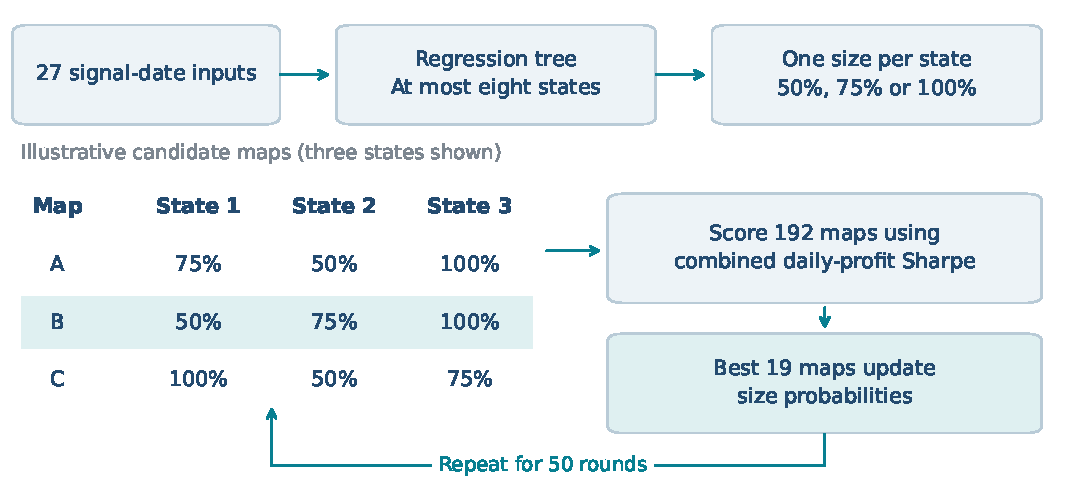
\includegraphics[width=\textwidth,height=242pt,keepaspectratio]{paper/unified_learning_2026_10_16/figures/entry_policy.pdf}\caption{The original tree/CEM construction. The three-state maps illustrate candidates; actual trees have up to eight states. Each candidate selects action-specific completed paths; the best 19 update sampling probabilities. The retained map sizes next month's proposals.}\end{figure}
For completed example i, p denotes its profit above cash on day d at size a. Each size has its own rounded contracts and simulated hedge path. A map assigns one size to each tree state. We sum its daily paths, retaining overlapping positions and zero-profit sessions, and score the result:

\[g_d(m)=\sum_i p_{i,d}(a_{\ell(x_i)}),\qquad\widehat S_{\rm train}(m)=\sqrt{252}\,\overline{g}/s_g.\]
CEM [3] updates size probabilities toward the best 19 of 192 candidate maps for 50 rounds. Constant maps and the incumbent are anchors. This standalone-path training score differs from funded-account Sharpe: replay additionally applies shared cash, inventory and admission.

\subsection*{Straddles: the same decision with ridge-score contexts}
The straddle bandit fits a 60-month ridge model to completed full-size profit, using 14 inputs and requiring 128 examples. The inputs include IV, RV-IV memory, VIX and a separate fixed-half paper portfolio's recent performance. Score terciles define three states. We enumerate all 27 size maps and retain the highest training Sharpe. Insufficient history uses half size. Both learners use completed outcomes; Appendix B provides exact fitting details.

\clearpage
\section*{12. Does learned entry sizing improve returns?}
\begin{figure}[H]\centering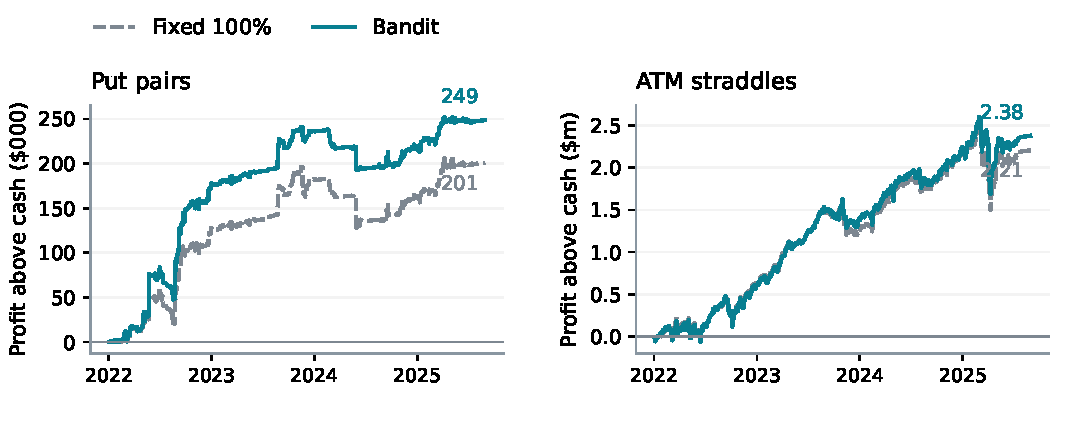
\includegraphics[width=\textwidth,height=235pt,keepaspectratio]{paper/unified_learning_2026_10_16/figures/entry_curves.pdf}\caption{Profit above cash since January 2022. Upper right: total straddle profits. Lower right: incremental straddle profit, bandit minus fixed full sizing. Series subtract their 2021 closing values and retain carried positions. Differences reflect both sizing and admission.}\end{figure}
\begin{center}\small\resizebox{\textwidth}{!}{\begin{tabular}{lllll}\toprule
Entry policy & 2018--21 S & 2022--25 S & Later entries & Later profit\\\midrule
Put pair · 50\% & 0.437 & 1.007 & 151 & \$0.205m\\
Put pair · 75\% & 0.449 & 0.944 & 104 & \$0.195m\\
Put pair · 100\% & 0.478 & 1.055 & 75 & \$0.201m\\
Put pair · Bandit & 0.573 & 1.263 & 110 & \$0.249m\\
Straddle · 50\% & 0.740 & 0.920 & 1782 & \$1.824m\\
Straddle · 75\% & 0.542 & 0.968 & 1222 & \$2.010m\\
Straddle · 100\% & 0.528 & 0.990 & 940 & \$2.206m\\
Straddle · Bandit & 0.775 & 1.041 & 1204 & \$2.379m\\
\bottomrule\end{tabular}}\end{center}
The put bandit improves later excess Sharpe by 0.208 and profit above cash by approximately \$47,800 relative to full size. It admits 110 entries instead of 75. The straddle bandit reaches Sharpe 1.041 and \$2.379 million above cash, compared with 0.990 and \$2.206 million at full size. Its earlier Sharpe also exceeds each fixed-size control. Straddles produce much more dollar profit and daily volatility than the put-pair portfolio, making allocation between them economically consequential.

These are comparisons of complete funded policies. All entry policies receive the same proposal pool---608 put-pair proposals and 35,774 straddle proposals---but size changes contract rounding, outstanding risk and the capacity to admit later opportunities. The resulting entries therefore differ. The findings support useful historical exposure choices; they do not isolate predictive sizing from admission effects.

Most of the put learner's later lead develops in 2022, while 2024 loses ground. Its annualized total account return is 4.667\%; growth relative to cash is 0.530\%. Average reserve is 2.44\% and peak reserve 15.77\%. Cash interest explains much total growth; trading value is measured above cash.

\clearpage
\section*{13. Explaining the bandits' decisions}
\begin{figure}[H]\centering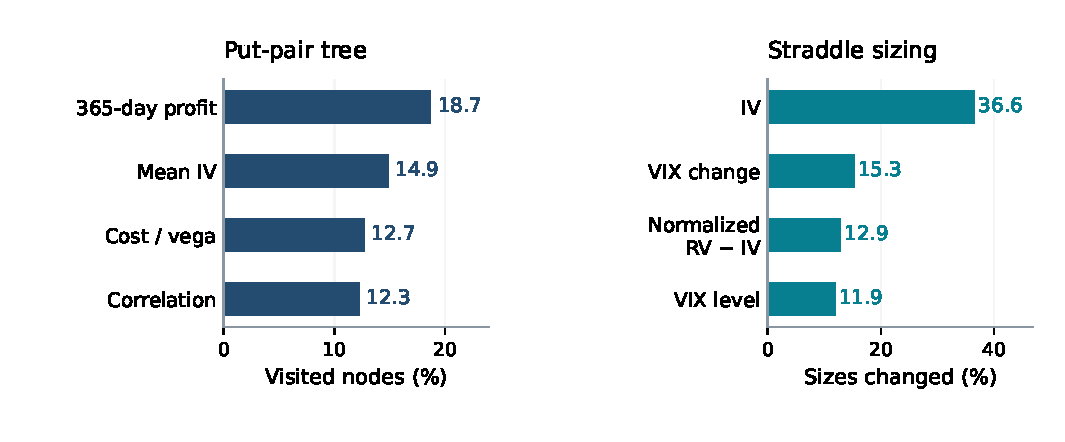
\includegraphics[width=\textwidth,height=213pt,keepaspectratio]{paper/unified_learning_2026_10_16/figures/entry_explanations.pdf}\caption{Put bars show the share of visited tree nodes; straddle bars show size changes when one input is centered. The denominators differ. Both are descriptive policy-usage measures.}\end{figure}
\subsection*{From an input to a requested trade size}
For a put proposal, interpretation is exact: follow the saved tree's root-to-leaf conditions, then read the size assigned to that leaf. Completed 365-day profitability appears in 18.7\% of later visited decision nodes, mean IV in 14.9\%, commission relative to vega in 12.7\%, and stock-return correlation in 12.3\%. These frequencies describe which information the fitted policy uses; they are not causal effects or a ranking of expected profit contributions.

For a straddle proposal, standardized ridge contributions add to a score. Saved thresholds locate its context, and the learned map selects a size. Centering IV changes 36.6\% of later fitted proposal sizes. Recent VIX change changes 15.3\%, normalized RV-minus-IV memory 12.9\%, and VIX level 11.9\%. The size map need not rise monotonically with the regression score because it optimizes the combined daily path. Exact replay reproduces every saved size across all 608 put and 35,774 straddle proposals.

\begin{center}\small\resizebox{\textwidth}{!}{\begin{tabular}{llll}\toprule
Later entry overlap vs full & Both & Bandit only & Fixed only\\\midrule
Put pairs & 74 & 36 & 1\\
Straddles & 897 & 307 & 43\\
\bottomrule\end{tabular}}\end{center}
Admission provides a second explanation for performance. Against fixed full size, the put bandit enters 36 later opportunities that the fixed policy rejects and misses one that it accepts. For straddles, those counts are 307 and 43. These differences can arise through the inventory left by earlier size decisions. An explanation of proposed size alone therefore does not explain the entire portfolio result.

Among quote-available completed straddle labels, full-size profit averages \$1,631 for proposals assigned full size and \$16 for those assigned half size. This subset is conditioned on available labels. Three within-date size shuffles yield later Sharpes 0.834, 0.928 and 1.044, versus 1.041 learned. One shuffle wins: favorable funded results and feature usage do not by themselves establish predictive sizing.

\clearpage
\section*{14. Q-learning allocates capital across signals}
The outer learner makes a different decision: what fraction of one \$10 million budget should track each funded strategy? Its seven put/straddle targets are 100/0, 90/10, 75/25, 50/50, 25/75, 10/90 and 0/100. Weights sum to one; there is no outer leverage or cash action. A weekly decision based on prior-close information takes effect at the next close. The first session retains old holdings, then positions resize and drift until the next decision.

\subsection*{State, action and action-dependent holdings}
Nine state inputs describe four economic opportunities---put-spread rank strength, the put implied-versus-realized variance gap, straddle IV-versus-RV richness and completed straddle premium---plus relative strategy volatility, strategy-return correlation, VIX, relative recent Sharpe and previous straddle weight. Previous holdings matter because changing allocations incurs additional costs. A target is a fractional claim on a funded strategy index, not a new integer-contract order book. Underlying trading costs remain embedded in source returns; resizing adds source-based option and hedge charges.

\[R_w(\lambda)=\sum_{d\in w}(z_d-\lambda z_d^2),\qquad z_d=e_d/\widehat{\sigma}_{\mathrm{ref}}\]
\subsection*{Reward and continuation value}
Reference volatility is estimated from the training window's fixed-50/50 excess returns. The parameter \ensuremath{\lambda} penalizes squared normalized fluctuations. At \ensuremath{\lambda} = 0, the directive is profit alone: additional normalized return earns reward without an explicit charge for the accompanying volatility. A higher-profit, higher-variance strategy can therefore attract capital even when its risk-adjusted performance is weaker. This objective does not maximize Sharpe. The discount \ensuremath{\gamma} = 0.99 separately weights continuation value; it is unchanged across risk preferences.

Monthly fitted Q iteration uses the preceding 104 completed weeks, with at least 52. A quadratic function of straddle weight has coefficients linear in standardized state, giving 30 coefficients. Each Bellman update regresses immediate reward plus discounted next-state maximum value onto the same basis [4]. We use ridge coefficient 10 and 200 updates. Seven prior allocations crossed with seven actions supply counterfactual paths on each market week; they do not create independent market observations.

Q uses 50/50 before enough training weeks exist; each fixed control starts at its own target. A discount-zero learner supplies a matched one-period control. In the factorial experiment, Q is refitted independently for each entry policy. Strategy-dependent risk features, reward paths and resizing charges are rebuilt for that policy, while economic signal definitions remain shared.

This outer experiment addresses an extension proposed in the original paper: freeze each signal's proposals, then learn how to combine their exposures. Entry sizes change the inner funded portfolios; Q changes the capital assigned across them. The accounting layers are deliberately distinct, allowing us to remove either learning layer in the four-way comparison.

\clearpage
\section*{15. Risk preference changes the allocation tradeoff}
\begin{figure}[H]\centering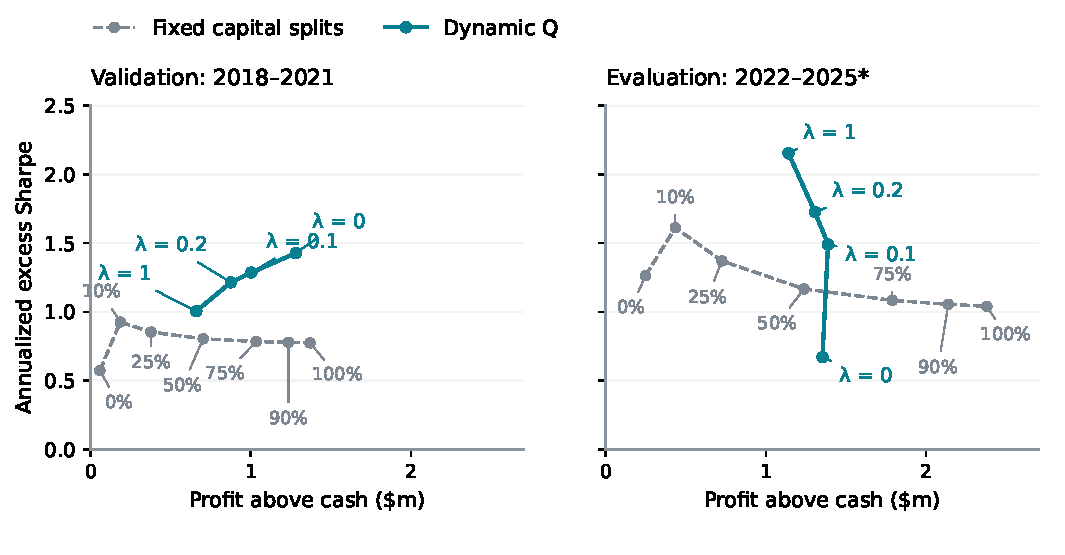
\includegraphics[width=\textwidth,height=267pt,keepaspectratio]{paper/unified_learning_2026_10_16/figures/allocation_risk.pdf}\caption{Bandit-managed source portfolios; nine-input Q state and \ensuremath{\gamma} = 0.99. Gray labels are fixed straddle percentages; the remainder goes to put pairs. Lines connect discrete policies. Both axes have the same scales across periods; 2025 ends in August.}\end{figure}
\begin{center}\small\resizebox{\textwidth}{!}{\begin{tabular}{lllll}\toprule
Reward & 2018--21 S & 2018--21 profit & 2022--25 S & 2022--25 profit\\\midrule
\ensuremath{\lambda} = 0 & 1.427 & \$1.281m & 0.671 & \$1.353m\\
\ensuremath{\lambda} = 0.1 & 1.286 & \$1.003m & 1.491 & \$1.388m\\
\ensuremath{\lambda} = 0.2 & 1.215 & \$0.875m & 1.726 & \$1.306m\\
\ensuremath{\lambda} = 1 & 1.005 & \$0.660m & 2.152 & \$1.141m\\
\bottomrule\end{tabular}}\end{center}
With bandit entries and \ensuremath{\lambda} = 0.20, Q reaches later Sharpe 1.726 and \$1.306 million profit above cash. Fixed 50/50 gives 1.167 and \$1.238 million; the highest-Sharpe fixed split, 90/10, gives 1.612 and \$435,181. At \ensuremath{\lambda} = 1, Q trades some profit for Sharpe 2.152. Straddle-heavy fixed allocations still generate more dollars. The curve therefore describes a profit--risk tradeoff, not dominance on every objective. At \ensuremath{\lambda} = 0.20, annualized growth relative to cash is 2.34\% and excess volatility 1.35\%; at \ensuremath{\lambda} = 1 these are 2.13\% and 0.98\%.

At \ensuremath{\lambda} = 0, the learner aggressively pursues profit through the higher-dollar, higher-variance straddle strategy. It chooses straddles alone in 138 of 191 later decisions, with a mean straddle target of 73.2\%, versus 24.9\% at \ensuremath{\lambda} = 0.20 and 16.9\% at \ensuremath{\lambda} = 1. Validation Sharpe is 1.427, but later Sharpe falls to 0.671. When straddle performance weakens, this concentration becomes costly: the zero-penalty portfolio loses approximately \$331,000 above cash in 2025.

The problem also involves when capital is committed. A fixed 75\% allocation to straddles achieves later Sharpe 1.084, so average exposure alone does not explain the weaker Q result. The profit-only learner can respond to state, but its learned timing does not distinguish attractive straddle opportunities well enough in the later period. Positive penalties make large fluctuations costly and lead to more selective straddle exposure. Increasing Bellman updates from 200 to 500, 1,000 and 2,000 changes no later decision for these settings. This check points to the reward and learned allocation rule, rather than too few iterations.

\clearpage
\section*{16. When does Q choose the riskier signal?}
Straddles offer more dollar profit and much greater daily risk. At \ensuremath{\lambda} = 0.20, Q chooses put pairs alone on 141 later decision dates, straddles alone on 46, and an interior mix on four. It primarily switches strategies.

\begin{figure}[H]\centering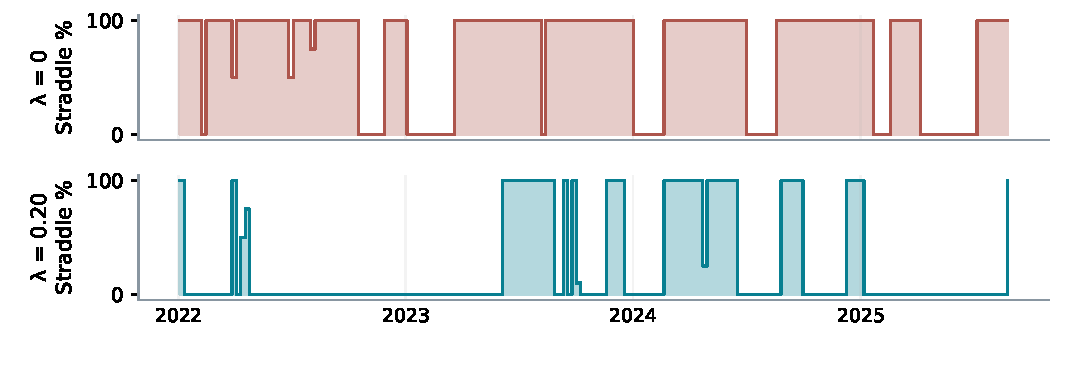
\includegraphics[width=\textwidth,height=159pt,keepaspectratio]{paper/unified_learning_2026_10_16/figures/allocation_schedule.pdf}\caption{Weekly target decisions during evaluation, before next-close execution. The remaining weight goes to put pairs. These are requested strategy allocations, not drifted portfolio holdings or individual trade sizes.}\end{figure}
\subsection*{The selected intervals have different carry-to-risk ratios}
\begin{figure}[H]\centering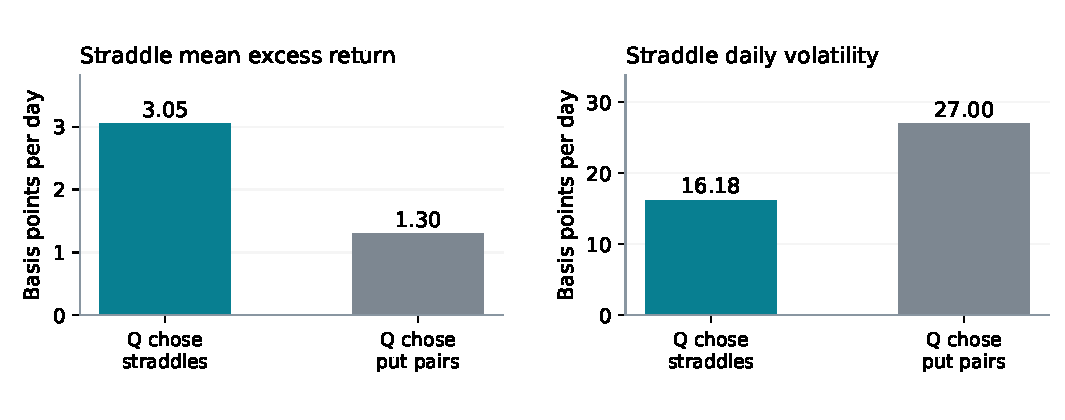
\includegraphics[width=\textwidth,height=202pt,keepaspectratio]{paper/unified_learning_2026_10_16/figures/conditional_risk.pdf}\caption{Realized straddle returns after \ensuremath{\lambda} = 0.20 Q decisions. Straddle-only choices cover 220 sessions; put-only choices cover 678. The four mixed-allocation intervals are omitted. Source costs are included; outer resizing charges are excluded.}\end{figure}
After Q chooses straddles, their mean daily excess return is 3.05 basis points with volatility 16.18; after it chooses put pairs, the straddle figures are 1.30 and 27.00. Put pairs average -0.09 basis points on the first set and +0.31 on the second. These are realized conditional statistics on noncontiguous dates, not causal estimates or standalone strategy Sharpes. Source costs are included; outer resizing charges are excluded.

A fixed target equal to Q's realized mean allocation reaches later Sharpe 1.387, versus 1.726 for Q: average exposure alone does not reproduce the result. The matched discount-zero learner reaches 1.645; continuation changes nine of 191 decisions at the same states. Much of the gain comes from conditional allocation, with a smaller incremental sequential benefit.

\clearpage
\section*{17. Separating the two learning layers}
\begin{figure}[H]\centering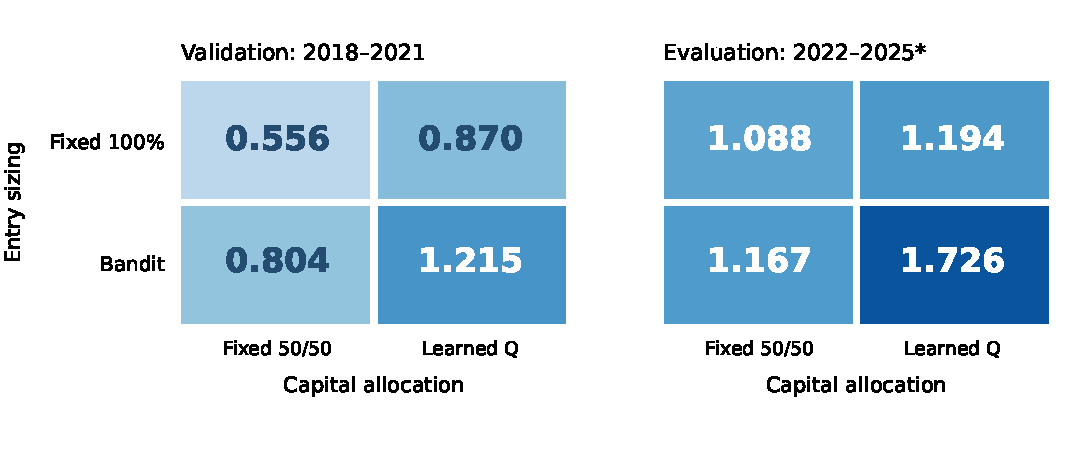
\includegraphics[width=\textwidth,height=216pt,keepaspectratio]{paper/unified_learning_2026_10_16/figures/factorial.pdf}\caption{Cell values are annualized excess Sharpe at \ensuremath{\lambda} = 0.20. Fixed entry size is 100\%; fixed capital allocation is 50/50. Q is independently fitted on each entry family's actual returns and costs.}\end{figure}
\begin{center}\small\resizebox{\textwidth}{!}{\begin{tabular}{llll}\toprule
Entry / capital policy & 2018--21 S & 2022--25 S & Later profit\\\midrule
Fixed / fixed & 0.556 & 1.088 & \$1.145m\\
Bandit / fixed & 0.804 & 1.167 & \$1.238m\\
Fixed / Q & 0.870 & 1.194 & \$0.955m\\
Bandit / Q & 1.215 & 1.726 & \$1.306m\\
\bottomrule\end{tabular}}\end{center}
The primary four-way comparison fixes the baseline at full entry size and 50/50 capital allocation. Both learning layers improve Sharpe in both periods, with the largest point-estimate gain when combined. The Q policy on fixed-entry portfolios is trained on those portfolios' own completed returns; it is not transplanted from the bandit portfolios. Economic opportunity inputs stay shared, while relative performance, volatility, correlation and costs change with the actual source strategies.

\begin{center}\small\resizebox{\textwidth}{!}{\begin{tabular}{lllll}\toprule
Fixed-75\% entries & 2018--21 S & 2022--25 S & Later profit & Drawdown\\\midrule
Fixed 50/50 & 0.566 & 1.070 & \$1.053m & 3.16\%\\
Q, \ensuremath{\lambda} = .20 & 0.891 & 2.118 & \$1.060m & 0.43\%\\
\bottomrule\end{tabular}}\end{center}
The fixed-75\% result shows that capital allocation can help independently of entry learning. Q nearly doubles later Sharpe with similar profit and a much smaller drawdown. Its later Sharpe exceeds bandit-plus-Q at this \ensuremath{\lambda}, while its profit and validation Sharpe are lower. Bandit sizing therefore changes the available profit--risk tradeoff without dominating every constant entry size.

\clearpage
\section*{18. Comparing dynamic allocation methods}
A dynamic policy might outperform fixed weights simply by responding to recent returns. We therefore adapt the minimum-variance, maximum-Sharpe and mean--variance portfolio objectives of Caner et al. [5] to our two frozen bandit portfolios. This comparison asks whether Q improves on conventional dynamic allocation as well.

\subsection*{The same budget, opportunities and execution}
All methods choose among the same seven capital splits, use one \$10 million budget and pay the same source trading and additional resizing costs. Estimates use Q's preceding 104 completed weeks, with a minimum of 52, monthly refits and the same 50/50 warmup. Within each objective, 2018--2021 Sharpe selects sample covariance or linear Ledoit--Wolf shrinkage; that choice remains fixed for the later period. This adapts their objectives rather than replicating their stock screens, nonlinear shrinkage or 15-year estimation window.

\begin{center}\small\resizebox{\textwidth}{!}{\begin{tabular}{lllll}\toprule
Capital allocator & 2018--21 S & 2022--25 S & Later profit & Later \ensuremath{\sigma} (\%)\\\midrule
Fixed 50/50 & 0.804 & 1.167 & \$1.238m & 1.973\\
Minimum variance & 0.316 & 1.329 & \$0.284m & 0.438\\
Maximum Sharpe & 0.189 & 0.659 & \$0.353m & 1.154\\
Mean--variance, \ensuremath{\lambda} = .20 & 0.355 & 1.519 & \$0.452m & 0.619\\
Q, \ensuremath{\lambda} = .20 & 1.215 & 1.726 & \$1.306m & 1.353\\
Mean--variance, \ensuremath{\lambda} = 1 & 0.246 & 1.795 & \$0.439m & 0.519\\
Q, \ensuremath{\lambda} = 1 & 1.005 & 2.152 & \$1.141m & 0.985\\
\bottomrule\end{tabular}}\end{center}
All S columns are annualized excess Sharpe; later \ensuremath{\sigma} is annualized daily excess-return volatility. At \ensuremath{\lambda} = 0.20, Q raises later Sharpe from 1.519 to 1.726 and profit above cash from \$452,303 to \$1,305,940. At \ensuremath{\lambda} = 1, the corresponding figures are 1.795 versus 2.152 and \$439,118 versus \$1,141,251. Q also improves both measures at \ensuremath{\lambda} = 0.10 in both periods. These are portfolio comparisons, not equal-risk experiments: Q takes more realized risk.

\subsection*{Why the allocation rules differ}
The conventional rules summarize each trailing window with one mean and covariance estimate. Q also conditions on current volatility pricing, completed premium, VIX and relative strategy performance. At \ensuremath{\lambda} = 0.20, its mean later straddle target is 24.9\%, versus 12.7\% for mean--variance allocation. The selected intervals in Section 16 have higher subsequent straddle returns and lower volatility, supporting selective participation rather than average exposure alone.

Q changes targets 24 times later, versus eight for mean--variance allocation. Removing only outer resizing charges raises their Sharpes to 1.774 and 1.525; all source trading costs remain. Lower resizing fees therefore do not explain Q's advantage. The conventional rule uses centered variance, whereas Q penalizes the raw second moment and adds state and continuation value; identical \ensuremath{\lambda} values do not make these identical objectives.

The result has a clear exception: at \ensuremath{\lambda} = 0, conventional profit-only allocation reaches later Sharpe 1.041 and \$2.154 million above cash, versus Q's 0.671 and \$1.353 million. The literal 1\% monthly target used in [5] is infeasible under our allocation limits; its maximum-mean fallback is recorded separately. All 14 conventional cases and the fee diagnostics are retained in the companion results.

\clearpage
\section*{19. An extension: managing accumulated straddle exposure}
Entry sizing and strategy allocation leave a third question: should an existing option position be trimmed as risk accumulates? A separate experiment uses a \$10 million joint whole-contract account, fixed 90\% put / 10\% straddle budgets and half-size entries in both sleeves. It does not replace the bandit accounts or the fractional-index Q experiment above.

A nonnegative regression predicts the magnitude of next-session straddle-book market P\&L from gross straddle vega and the preceding 21-session RMS P\&L. The coefficients and a 75th-percentile risk-per-NAV cutoff use 2018--2021 data. Cuts are inactive then, so this fits the warning without validating the management rule. When the reference-book warning is high, new straddles pause and existing cohorts target half their original integer counts at the next close. Trims remain in place; put rules are unchanged. This is an interpretable risk rule, not a learned Q-management policy.

\begin{figure}[H]\centering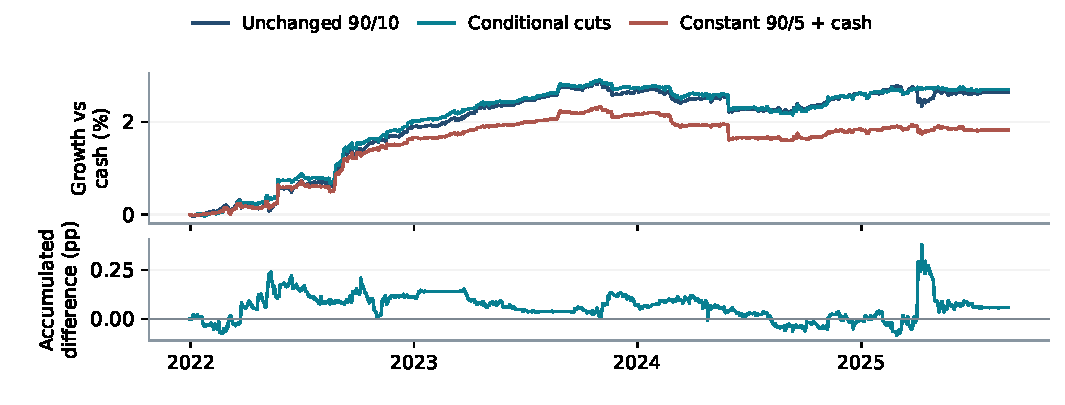
\includegraphics[width=\textwidth,height=200pt,keepaspectratio]{paper/unified_learning_2026_10_16/figures/straddle_management.pdf}\caption{Separate joint-contract management trial, January 2022--August 2025. Upper panel: compounded growth relative to cash. Lower panel: cumulative daily excess-return difference, conditional cuts minus unchanged 90/10. This is not the Q-index account.}\end{figure}
\begin{center}\small\resizebox{\textwidth}{!}{\begin{tabular}{lllll}\toprule
Account & Mean excess (\%) & Vol. (\%) & Sharpe & Drawdown (\%)\\\midrule
Unchanged 90/10 & 0.718 & 0.525 & 1.365 & 0.676\\
Conditional cuts & 0.733 & 0.465 & 1.576 & 0.734\\
Constant 90/5 + cash & 0.499 & 0.435 & 1.147 & 0.719\\
\bottomrule\end{tabular}}\end{center}
During January 2022--August 2025, conditional cuts raise excess Sharpe from 1.365 to 1.576, mainly by reducing volatility while preserving the arithmetic mean excess return. Cash-relative maximum drawdown becomes slightly worse, 0.734\% versus 0.676\%. The paired 126-session bootstrap interval for the Sharpe gain is -0.22 to +0.66. Annualized mean excess return is 252 times the daily mean, not compounded growth.

The constant-lower control assigns 90\% to puts, 5\% to straddles and 5\% to cash. It takes less average straddle exposure than the conditional policy, so it does not isolate timing at equal exposure. The trial motivates inventory-aware learning but does not establish that trimming reliably improves performance. The timing, exposure and reproduction details appear in Appendix F.

\clearpage
\section*{20. Interpretation, limitations and conclusion}
\subsection*{What the comparisons establish}
Entry bandits improve the retained portfolios through sizing and admission. Q improves allocation with constant entries and exceeds the corresponding rolling mean--variance controls at \ensuremath{\lambda} = 0.10, 0.20 and 1. Its profit-only policy transfers less reliably when straddles weaken. Reward design changes the allocation tradeoff.

\subsection*{What remains uncertain}
All fitted policies use only information available before their decisions. However, strategy development included inspection of later-period results, including choices of training windows and risk preferences. Consequently, the evaluation measures historical performance under chronologically fitted policies, rather than an independently frozen test of the complete research process. The controlled comparisons provide evidence about adaptive exposure allocation under the stated assumptions, but neither the magnitude of research-selection bias nor prospective performance has been established.

Execution is another boundary. Midpoint-based fills with an adverse charge do not establish tradability, particularly for paired orders that may fill asynchronously. Quoted-spread execution, liquidity capacity, pin risk, early assignment and forced liquidation need further work. The outer experiment reallocates fractional strategy indices, not shared integer contracts; the separate common-ledger trimming trial does not remove this limitation from the Q comparison. Initial vega matching is local, and the straddle signal adds net short-volatility risk.

\subsection*{Conclusion}
The two signals explain why capital allocation matters. Relative put pricing creates a low-deployment portfolio with favorable selected-period risk-adjusted returns. Persistent RV-IV selling earns more dollars with greater exposure to realized movement. Neither dominates for every investor. The allocation learner links these economic differences to a risk-preference reward and current information, extending the original question from one trade rule to competing sources of return.

The straddle attribution links the second signal to realized movement and explains why positive stock-hedge profits are not a separate edge. A joint-contract trimming trial supplies an interpretable inventory-management candidate, with an uncertain gain. Future work should integrate such controls with learned allocation, measured execution costs and additional independent signals.

Bandits adapt trade commitments; Q allocates across strategies. The four-way and conventional-benchmark comparisons support studying both exposure decisions in an integrated implementation and prospective evaluation.

\clearpage
\section*{References}
[1] Ning, B., and K. Lee (2024). Advanced Statistical Arbitrage with Reinforcement Learning. arXiv:2403.12180. https://arxiv.org/abs/2403.12180

[2] Goyal, A., and A. Saretto (2009). Cross-section of option returns and volatility. Journal of Financial Economics 94, 310--326. https://doi.org/10.1016/j.jfineco.2009.01.001

[3] de Boer, P.-T., D. P. Kroese, S. Mannor, and R. Y. Rubinstein (2005). A Tutorial on the Cross-Entropy Method. Annals of Operations Research 134, 19--67. https://people.smp.uq.edu.au/DirkKroese/ps/aortut.pdf

[4] Ernst, D., P. Geurts, and L. Wehenkel (2005). Tree-Based Batch Mode Reinforcement Learning. Journal of Machine Learning Research 6, 503--556. https://jmlr.org/papers/v6/ernst05a.html

[5] Caner, M., A. Capponi, N. Sun, and J. Y. Tan (2026). Designing Agentic AI-Based Screening for Portfolio Investment. arXiv:2603.23300. https://arxiv.org/abs/2603.23300

[6] Bell, S., A. Kakhbod, M. Lettau, and A. Nazemi (2026). AlphaGlass: Interpretable Characteristic-Based Portfolio Choice. NBER Working Paper 35186. https://doi.org/10.3386/w35186

\clearpage
\appendix
\section*{Appendix A. Contracts, features and account checks}
\subsection*{Data and trade construction}
WRDS supplies option quotes, stock prices, rates and distributions. The inherited formation archive contains 345 pairs; 125 prepared pairs with 161 equity/ETF underlyings supply candidates. Forty-six pairs generate 608 screened put proposals over 2018--2025. This universe is retrospective and conditioned on usable coverage. The companion roster in paper/pair\_universe.csv records prepared pairs and candidate-date ranges, which are not claims of continuous quote availability.

Put selection takes the expiry nearest 30 days, then the put nearest absolute delta 0.25 within 0.075. Ties prefer narrower quotes, higher open interest and lower contract identifier. Entry requires standard 100-share contracts, positive noncrossed quotes, open interest of at least 100, quote width no more than 25\% of midpoint and 7--55 days remaining. Straddles match call and put on name, strike, expiry and adjustment. Corporate events can force exits; missing entry quotes reject proposals. Held marks may use last-known IV with current spot, rates and known dividends.

\subsection*{Entry-state definitions}
\begin{center}\small\resizebox{\textwidth}{!}{\begin{tabular}{ll}\toprule
Put-pair feature group & Numerical inputs\\\midrule
Volatility and opportunity & Mean IV; oriented IV gap; rank strength; oriented IV\ensuremath{^2}-minus-trailing-variance gap; mean RV\\
Relatedness and maturity & 126-session beta and correlation; mean expiry and expiry difference\\
Costs and market & Training commission in IV points; strictly prior VIX close\\
Completed profitability & 91-day and 365-day mean profit per initial vega and completed counts\\
\bottomrule\end{tabular}}\end{center}
These are 15 numerical inputs. The first three are core fields; the remaining 12 have binary availability flags, giving 27 inputs. Missing optional values are zero with flag zero. Put trailing variance is 252 times mean squared simple stock returns over 20 sessions, with at least 10 observations. The straddle signal uses annualized squared log returns and a 21-session RV input. The measures have different retained definitions; no new common RV estimator is fitted for this comparison.

The straddle's 14 ridge inputs are completed residual memory, IV, VIX, normalized memory, variance ratio, 21-session VIX change, 5-session IV change, and a fixed-half benchmark's 21/63/126-session Sharpe, 63-session volatility and drawdown, reserve use and availability flag. These benchmark states come from an external causal paper portfolio, not the learner's own future inventory.

\subsection*{Admission and risk accounting}
Research stress takes each name's worst modeled option-plus-hedge loss across spot shocks -20/0/+20\% and IV shocks -10/0/+10 points, then sums without pair-correlation credit. Limits are stress loss 5\% of budget, reserve 80\%, hedge notional twice budget and gross vega \$20,000 per IV point per \$1 million. Reserve is gross option premium plus half netted hedge notional. Global checks use equity; pair checks use a \$1 million reference scaled by current/initial equity. These are research limits, not broker margin. European-style valuation and cash settlement approximate expiry; assignment is not fully simulated.

\clearpage
\section*{Appendix B. Fitting, chronology and controls}
\subsection*{Entry optimizers}
The put tree has up to eight leaves, with minimum count max(8, min(63, floor(n/8))); fewer than 16 examples use full size. CEM uses 50 rounds of 192 maps, 19 elites and seed 2026. Probabilities start uniform; updates mix 30\% prior probability and 70\% elite frequency, shrink by 0.97 and add 0.03 uniformly. Constant maps and the incumbent are anchors. Separate rounded-contract paths supply daily training profits; funded NAV returns supply evaluation Sharpe. Put memory and training labels retain a \$0.65 option commission; funded evaluation uses \$0.03 for every policy.

The straddle ridge fit uses median centers, standard deviations floored at 0.001, clipped inputs within \ensuremath{\pm}5, penalty 100 with no intercept penalty, and equal total weight per date. Full-size completed profit is its target. Score terciles define contexts; all 27 size maps are evaluated on aggregate daily paths. Ties favor lower exposure. The 60-month window requires 128 examples. Only 4,116 training rewards are finite; the policy still handles all 35,774 proposals.

\subsection*{Q specification and numerical check}
\[Q(s,a)=b(s)+a\,c(s)+a^2d(s),\qquad a\in\{0,.10,.25,.50,.75,.90,1\}\]
Each coefficient function is linear in the intercept and nine standardized inputs. Training centers use means, scales have floor 0.1, and standardized values are clipped within \ensuremath{\pm}5. Ridge is 10, except the global intercept penalty 0.01. Bellman regression weights counterfactual rows so each week has unit total mass. The reference volatility is that family's completed-window 50/50 daily excess standard deviation. All 81 monthly fits were checked at 200, 500, 1,000 and 2,000 updates. Later actions are identical across budgets for the four reported \ensuremath{\lambda} values.

\begin{center}\small\resizebox{\textwidth}{!}{\begin{tabular}{llll}\toprule
Allocation control, \ensuremath{\lambda} = .20 & 2018--21 S & 2022--25 S & Later profit\\\midrule
Fixed at Q's mean target & 0.828 & 1.387 & \$0.841m\\
One-period learner, \ensuremath{\gamma} = 0 & 1.053 & 1.645 & \$1.184m\\
Sequential Q, \ensuremath{\gamma} = 0.99 & 1.215 & 1.726 & \$1.306m\\
\bottomrule\end{tabular}}\end{center}
The mean-weight control uses the realized average target retrospectively. Forty-nine nonzero circular rotations of the saved \ensuremath{\lambda} = 0.20 action schedule preserve its action counts and most serial structure; none reaches actual later Sharpe, while three reach or exceed actual validation Sharpe. Their median later Sharpe is 0.744. Wealth and resizing costs are recomputed. These are descriptive timing diagnostics, not selection-adjusted tests.

\subsection*{Chronology and statistical interpretation}
Every fit uses strictly completed past outcomes. Put selection ranks 33 archived screened configurations by 2018--2021 scores before the \$10 million replay. The straddle's 48- and 60-month windows tie at validation Sharpe 0.775; later Sharpes of 0.960 and 1.041 informed refinement. The four displayed Q preferences illustrate researched risk choices, not a single validation-winning policy. The original selection and full results remain in reports/signal\_allocation\_discount. The put-sizing gain is 0.208, with a paired 95\% interval of -0.103 to +0.424, using 1,000 circular resamples of 126-session blocks, fixed policies and no selection adjustment. These records identify research choices without measuring their bias.

\clearpage
\section*{Appendix C. Supporting results and reproducibility}
\begin{center}\small\resizebox{\textwidth}{!}{\begin{tabular}{lllll}\toprule
Year & Put bandit & Straddle bandit & Q: \ensuremath{\lambda} = .20 & Q: \ensuremath{\lambda} = 1\\\midrule
2018 & 0.522 & 0.148 & 0.160 & 0.160\\
2019 & -0.542 & 1.459 & 0.112 & -0.237\\
2020 & 1.555 & 0.161 & 1.617 & 1.028\\
2021 & -0.580 & 2.336 & 2.932 & 3.180\\
2022 & 2.458 & 1.206 & 2.042 & 2.540\\
2023 & 1.492 & 1.727 & 2.449 & 2.907\\
2024 & -0.907 & 1.465 & 1.945 & 1.954\\
2025* & 1.092 & 0.085 & -0.598 & 1.092\\
\bottomrule\end{tabular}}\end{center}
All figures are annualized excess Sharpe; 2025 ends on 29 August. The sleeves retain their separate funded histories, and outer allocations include resizing charges. Annual results show regime variation that aggregate ratios conceal. A high pooled Sharpe is not evidence of positive excess performance every year.

\begin{center}\small\resizebox{\textwidth}{!}{\begin{tabular}{lllll}\toprule
Entry policy + Q & \ensuremath{\lambda} = 0 & \ensuremath{\lambda} = .10 & \ensuremath{\lambda} = .20 & \ensuremath{\lambda} = 1\\\midrule
Fixed 50\% & 0.541 & 0.703 & 1.116 & 1.349\\
Fixed 75\% & 0.606 & 0.667 & 2.118 & 1.897\\
Fixed 100\% & 0.618 & 1.354 & 1.194 & 1.633\\
Bandit & 0.671 & 1.491 & 1.726 & 2.152\\
\bottomrule\end{tabular}}\end{center}
This table holds Q's feature definitions, discount, training window and action menu fixed while refitting separately on each entry family. Values are 2022--2025 Sharpes. The complete seven fixed capital splits are also retained; 50/50 is the primary fixed-allocation baseline, rather than a later-period optimized control.

\subsection*{Evidence and reproduction}
Entry results come from reports/p25\_validation\_split/periods.csv and reports/straddle\_policy\_refinement/comparison.csv. Exact entry explanations are in reports/retained\_entry\_explanations. Allocation results, decisions and convergence checks are in reports/signal\_allocation\_variance. Independent fixed-entry Q fits and the four-way experiment are in reports/signal\_learning\_factorial. Its checks reproduce all eight pure strategy endpoints and 324 monthly checkpoint timings. The paper's provenance manifest records source and figure hashes.

The companion scripts preserve the actual-contract ledger and the separate fractional-index allocator. Model fitting requires the licensed source cache or archived derived inputs; vendor redistribution restrictions still apply. Reproduce this document from its saved manuscript and figures without refitting any model. Public repository: https://github.com/kreitzz/rl-atm-vega-pairs

\clearpage
\section*{Appendix D. Original sizing and annual results}
\subsection*{Alternative put sizing pipelines retained from the original study}
\begin{center}\small\resizebox{\textwidth}{!}{\begin{tabular}{lllll}\toprule
Put sizing policy & 2018--21 S & 2022--25 S & Later entries & Later profit\\\midrule
Constant 50\% & 0.437 & 1.007 & 151 & \$0.205m\\
Constant 75\% & 0.449 & 0.944 & 104 & \$0.195m\\
Constant 100\% & 0.478 & 1.055 & 75 & \$0.201m\\
Tree + CEM & 0.573 & 1.263 & 110 & \$0.249m\\
Spread-rank sizing & 0.464 & 0.815 & 121 & \$0.165m\\
Ridge-score sizing & 0.421 & 0.890 & 94 & \$0.180m\\
Direct linear policy & 0.267 & 0.873 & 96 & \$0.171m\\
Direct additive policy & 0.302 & 1.013 & 97 & \$0.180m\\
\bottomrule\end{tabular}}\end{center}
All policies receive the same put proposals, directions, contracts and funded admission rules. The lower four rows are follow-up comparisons rather than original selection candidates. Tree/CEM has the highest funded Sharpe in both periods among these policies. These comparisons retain the original question about entry sizing alongside the newer straddle and allocation experiments.

\begin{center}\small\resizebox{\textwidth}{!}{\begin{tabular}{lllll}\toprule
Year & Account return & Above cash (pp) & Excess Sharpe & Entries\\\midrule
2022 & 3.470\% & 1.673 & 2.458 & 66\\
2023 & 5.288\% & 0.432 & 1.492 & 19\\
2024 & 5.104\% & -0.283 & -0.907 & 11\\
2025* & 3.207\% & 0.169 & 1.092 & 14\\
\bottomrule\end{tabular}}\end{center}
Calendar-period account returns and above-cash differences are not annualized, including partial 2025. Sharpe is annualized. In 2024 the account grows while losing relative to cash. The original put strategy's results are concentrated in a few pairs and in 2022; this limits claims of broad repeated success.

The original put results are concentrated: SNAP/UBER, GAP/TJX and AMD/MU contribute 66.9\% of later net pair trading profit, and 2022 supplies 83.1\%. These figures exclude shared financing. They describe where gains occurred, not a rule for selecting those names retrospectively. Annual Sharpe ratios are retained in Appendix C.

The put account's later annualized total account return is 4.667\%, versus 0.530\% growth relative to cash. Average reserve is 2.44\% and peak reserve 15.77\%. Its cash-relative drawdown is 0.495\%, compared with 0.646\% at full size. These figures retain the original distinction between a profitable trading signal, account funding and capital deployment.

\clearpage
\section*{Appendix E. Performance definitions and timing diagnostics}
\subsection*{Account return, cash-relative growth and dollar profit}
Let N be account NAV and K the continuing all-cash benchmark. Both begin at \$10 million in January 2018. The benchmark compounds the previous available WRDS zero-curve rate nearest 30 days over calendar days using a 365-day year. For each reporting period, 0 is the preceding close and T the final close.

\[e_t=\frac{N_t}{N_{t-1}}-\frac{K_t}{K_{t-1}},\qquad\widehat S=\sqrt{252}\,\overline{e}/s_e.\]
Dollar profit above cash is (N\_T - K\_T) - (N\_0 - K\_0). With Q\_t = N\_t/K\_t and Y equal to elapsed days divided by 365.25, annualized growth relative to cash is (Q\_T/Q\_0)^(1/Y) - 1. Cash-relative drawdown is the greatest percentage decline of Q from its running peak, including the opening close. The annual table instead subtracts the cash return from the account return, in percentage points.

At the 2021 close, the learned put account has \$10.568 million equity and four open trades; full sizing has \$10.581 million and three. Cash benchmark wealth is \$10.510 million. Performance curves subtract each policy's opening dollar excess wealth; they do not reset accounts or liquidate inventory at the reporting split.

\subsection*{Additional allocation diagnostics}
Centering VIX and straddle IV-versus-RV richness changes 13.6\% and 12.6\% of later actions. Across 49 nonzero rotations of Q's saved schedule, none reaches its later Sharpe; median Sharpe is 0.744. These diagnostics explain information use and timing, without establishing causal feature effects or selection-adjusted significance.

The rotation control preserves allocation counts and most serial structure, then recomputes wealth and resizing costs. Three of 49 rotated schedules reach or exceed the actual validation Sharpe; none reaches the actual later Sharpe. Timing-control results are reported in Appendix B. These are diagnostics of the retained policy, not a substitute for prospective evaluation.

A final distinction concerns portfolio admission. The source put and straddle books each simulate whole contracts and daily stock hedges under their own funded histories. The outer allocator trades fractional claims on those net strategy indices, with additional resizing charges. Its capital weights are not premium deployment or broker margin, and reallocating indices does not rerun a common integer-contract inventory ledger.

\clearpage
\section*{Appendix F. Straddle attribution and management protocol}
\subsection*{Retained cohorts and accounting checks}
The economics extension retains 2,599 unique straddle cohorts and reconciles their option-plus-stock profits to the full-history straddle account. The aggregate bridge includes \$160,755 in hedge trading costs, \$20,544 in short-stock borrow, \$57,201 in hedge dividends and \$498,494 in cash interest above the cash benchmark. Option charges are already included in the option component. These amounts belong to January 2018--August 2025, not only the later reporting period.

Saved holdings and recovered quote paths reproduce the trade illustrations. One quote-availability convention was inferred; using observed recovered quotes changes aggregate hedge profit by \$367.52. The figures retain the reconciled saved-account attribution. This reconstruction difference is disclosed rather than counted as a new profit source. Stable security identifiers identify the two examples.

\subsection*{Risk warning and executable trimming}
The warning model uses nonnegative coefficients 1.405401 on gross straddle vega and 0.383233 on 21-session RMS market P\&L. Divide its dollar prediction by prior NAV and compare with 0.0001616954. The predictor targets absolute next-session market P\&L, not its sign. A causally maintained unchanged reference book supplies the state, so a trim cannot mechanically switch off its own warning.

A high warning pauses new straddles and requests 50\% of each original cohort's call and put counts, rounded down. One-contract cohorts close both legs. The target is retried until filled or expired and never restores trimmed positions; new entries resume after the warning clears. The first signal is 31 December 2021, execution 3 January 2022, and first affected market return 4 January. All 908 warning records strictly order signal, execution and first affected return.

Mean later gross straddle vega is \$562.36 per volatility point for unchanged 90/10, \$450.59 for conditional cuts and \$275.54 for constant 90/5 plus cash. Thus the constant-lower control does not match average exposure. The saved paired bootstrap uses 2,000 draws; the Sharpe-gain interval versus holding is [-0.243, +0.697] at 63 sessions and [-0.218, +0.665] at 126. These intervals condition on the retained histories without research-selection adjustment.

\subsection*{Publication reproduction and experiment scope}
The committed reports/strategy\_economics/data snapshots and manifest reproduce the attribution, figures and management table without raw option chains. The renderer verifies snapshot hashes, cohort identities, aligned account dates and saved performance arithmetic. The original management simulator and model-fitting pipeline are not included in this focused publication snapshot; publication reproduction is not an independent regeneration of those experiments.

The three management accounts have identical histories before 2022, each with excess Sharpe 0.882. No cuts are applied during that period; it estimates the warning model and cutoff rather than validating the trimming benefit. Their later daily return and benchmark identities reconcile, including whole-contract exposure and funding in the saved ledgers. Other forecast, sizing and allocation variants were investigated without a replacement policy being retained. This one bounded trial uses already researched historical dates and is a separate extension, not a fresh holdout or additional evidence that the main Q learner manages individual contracts.

\end{document}
